\chapter{Grafos de Moore}
\label{moore}

Estudando os grafos de diâmetro 2, percebemos alguns grafos que atendiam ao limite dado pelo Corolário \ref{coro-env-gd2} e pelo Teorema \ref{teor-d2-big-o-sr}. Por exemplo, o grafo $C_5$, grafo de Petersen e o grafo Hoffman-Singleton. Esses grafos são conhecidos como grafos de Moore. 

Um Grafo de {\it Moore} é um Grafo regular de grau $k$ e diâmetro $d$ tal que o número de vértices é igual ao limitante superior $$1 + d\sum_{i=0}{d-1}(k-1)^i$$

 Os grafos de Moore foram definidos por Hoffman e Singleton em \cite{Hoffman1960} onde concluíram que grafos de Moore de diâmetro 2, só são possíveis para os valores de $k$ igual a 2, 3, 7 ou 57. Sendo $k=2$ o grafo $C_5$, $k=3$ o grafo de Petersen, $k=7$ o grafo Hoffman-Singleton e o grafo $k=57$ que permanece desconhecido até então.

Mesmo desconhecido sabe-se que o grafo de Moore 57-regular deve possuir algumas propriedades já verificadas em outros trabalhos posteriores. Sabe-se que esse grafo possui ao menos 375 automorfismo \cite{Macaj2010}, não é vértice-transitivo \cite{Cameron1983,Miller2005} e tão pouco distância-transitivo \cite{Aschbacher1971,Miller2005}. Por fim pelas conclusões dos trabalhos de \cite{Bannai1973,Damerell1973}, não existem grafos de Moore tais que $\Delta \geq 3$ e $d\geq 3$, ou seja eles possuem diâmetro no máximo 2.

Permanece em aberto até hoje se existe o grafo de Moore 57-regular e diâmetro 2. Este grafo é conhecido como o último grafo de Moore.

Apesar de não termos conseguido determinar a existência do mesmo, nas implementações deste trabalho conseguimos avançar um pouco nessa busca. 


%EXPLICAR O FUNCIONAMENTO DE CADA ALGORTIMO

O Algoritmo \ref{alg-geracao-grafo-moore} possui duas etapas distintas, inicialmente um esqueleto do grafo é gerado e por fim arestas são adicionadas respeitando as restrições da regularidade e cintura do grafo objetivo.

Na primeira etapa é gerado um esqueleto do grafo contendo todos $k^2+1$ vértices, ou seja os vértices $v_0, v_1,..,v_{k^2}$ o algoritmo inicia a construção partindo de um caminho $P_3$ formado pelos vértices $v_{k^2-2}v_{k^2}v_{k^2-1}$. O vértice $v_{k^2-2}$ e $v_{k^2-2}$ possui outros $k-1$ vizinhos. Como trata-se de um grafo de Moore de diâmetro 2, por definição a cintura do grafo é 5, esses outros vizinhos são distintos dos demais vértices do $P_3$ inicial. Portanto podemos atribuir a vizinhança de $v_{k^2-2}$ os vértices de $v_0$ até $v_{k-2}$. Analogamente podemos atribuir a vizinhança de $v_{k^2-1}$ os vértices de índice $k-1$ até $2k-3$. 

Com o passo anterior concluído, temos todos os $k$ vizinhos de $v_{k^2-2}$ e $v_{k^2-2}$, sabemos que em um grafo de diâmetro 2 a vizinhança de todo vértice é um conjunto dominante, então cada vizinho de $v_{k^2-2}$ precisar ter uma aresta para algum vizinho de $v_{k^2-1}$, sem perda de generalidade podemos estabelecer as arestas $(v_0,v_{k-1})$, $(v_1,v_k)$, ..., $(v_{k-2},v_{2k-3})$.


\begin{figure}[h]
\centering
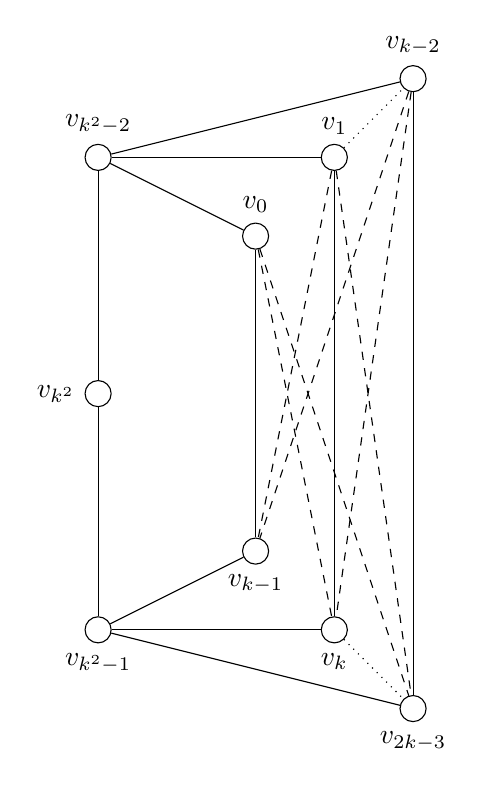
\begin{tikzpicture}
\node[circle,draw,label=$v_{k^2-2}$] (v2) at (-2.5,3) {};
\node[circle,draw,label=$v_{0}$]   (v4) at (-0.5,2) {};

\node[circle,draw,label=left:$v_{k^2}$]  (v1) at (-2.5,0) {};
\node[circle,draw,label=below:$v_{k^2-1}$]  (v3) at (-2.5,-3) {};
\node[circle,draw,label=below:$v_{k-1}$]  (v7) at (-0.5,-2) {};

\node[circle,draw,label=$v_{1}$]  (v5) at (0.5,3) {};
\node[circle,draw,label=$v_{k-2}$]  (v6) at (1.5,4) {};
\node[circle,draw,label=below:$v_{k}$]  (v8) at (0.5,-3) {};
\node[circle,draw,label=below:$v_{2k-3}$]  (v9) at (1.5,-4) {};

\draw  (v1) edge (v2);
\draw  (v1) edge (v3);
\draw  (v2) edge (v4);
\draw  (v2) edge (v5);
\draw  (v2) edge (v6);
\draw  (v3) edge (v7);
\draw  (v3) edge (v8);
\draw  (v3) edge (v9);
\draw  (v4) edge (v7);
\draw  (v5) edge (v8);
\draw  (v6) edge (v9);

%\node[circle,draw,label=$v_{0}$]  (v10) at (-1.5,0.5) {};
%\node[circle,draw,label=below:$v_{0}$] (v11) at (-1.5,-0.5) {};
%\draw  (v1) edge (v10);
%\draw  (v1) edge (v11);

\draw[dashed] (v4) edge (v8);
\draw[dashed]  (v5) edge (v7);
\draw[dashed]  (v6) edge (v7);
\draw[dashed]  (v4) edge (v9);
\draw[dashed]  (v5) edge (v9);
\draw[dashed]  (v6) edge (v8);

\draw[dotted]  (v5) edge (v6);
\draw[dotted]  (v8) edge (v9);
\end{tikzpicture}
\caption{Início da etapa-1 de geração do grafo de Moore}
\label{fig-execucao-moore}
\end{figure}

Em um grafo de diâmetro 2, todo par de vértice é adjacente ou possui um vizinho em comum. Seguindo essa propriedade vamos analisar individualmente a situação dos vértices $v_0$ até $v_{2k-3}$. Começando por $v_0$ podemos perceber que ele está em conformidade com o $P_3$ inicial, seu vizinho $v_{k-1}$ e seus irmãos $v_1,...,v_{k-2}$. Porém para um grafo de diâmetro 2, $v_0$ não está em conformidade com os vértices $v_k,v_{k+1},...,v_{2k-3}$. De forma análoga e espelhada podemos analisar o vértice $v_{k-1}$ que está em conformidade com  o $P_3$ inicial, seus vértices vizinhos e irmãos  conforme pode ser visto pelas linhas tracejadas na Figura~\ref{fig-execucao-moore}.

Dado que o grafo tem diâmetro 2 e cintura 5, as não conformidades dos vértices, listadas anteriormente, não podem ser resolvidas com adição de arestas entre eles. Então a única forma restante é um vizinho em comum. Portanto a não conformidade entre $v_0$ e $v_k$ será resolvida com um novo vértice $v_{2k-2}$ adjacente a ambos. De forma análoga a não conformidade de $v_{k-1}$ e $v_1$ será resolvida com um novo vértice $v_{2k-1}$. Assim sucessivamente com todos os demais vértices, serão criados então $(k-1).(k-2)$ novos vértices, que vão de $v_{2k-2}$ até $v_{k^2-k-1}$, conforme podemos ver na Figura~\ref{fig-execucao-moore-2}.

\begin{figure}[h]
\centering
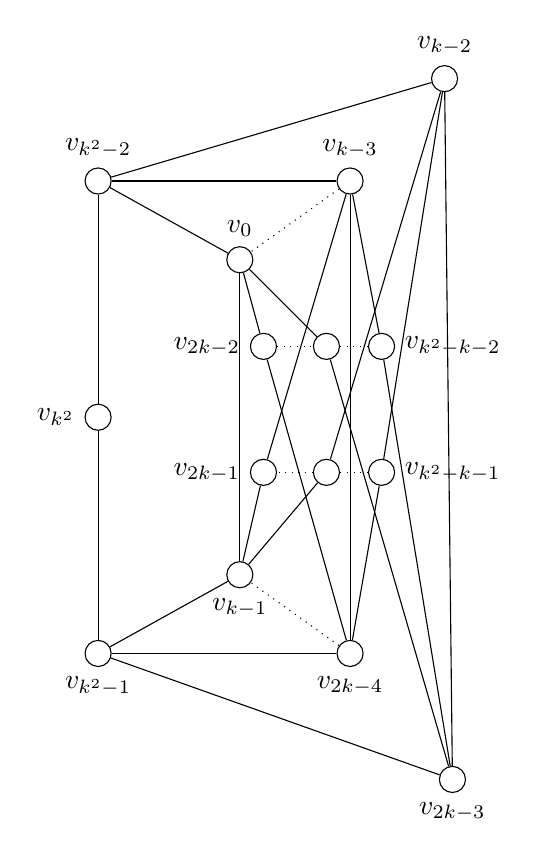
\begin{tikzpicture}
\node[circle,draw,label=$v_{k^2-2}$] (v2) at (-2.5,3) {};
\node[circle,draw,label=$v_{0}$] (v4) at (-0.7,2) {};

\node[circle,draw,label=left:$v_{k^2}$]  (v1) at (-2.5,0) {};
\node[circle,draw,label=below:$v_{k^2-1}$]  (v3) at (-2.5,-3) {};
\node[circle,draw,label=below:$v_{k-1}$] (v7) at (-0.7,-2) {};

\node[circle,draw,label=$v_{k-3}$] (v5) at (0.7,3) {};
\node[circle,draw,label=$v_{k-2}$] (v6) at (1.9,4.3) {};
\node[circle,draw,label=below:$v_{2k-4}$] (v8) at (0.7,-3) {};
\node[circle,draw,label=below:$v_{2k-3}$] (v9) at (2,-4.6) {};

\draw  (v1) edge (v2);
\draw  (v1) edge (v3);
\draw  (v2) edge (v4);
\draw  (v2) edge (v5);
\draw  (v2) edge (v6);
\draw  (v3) edge (v7);
\draw  (v3) edge (v8);
\draw  (v3) edge (v9);
\draw  (v4) edge (v7);
\draw  (v5) edge (v8);
\draw  (v6) edge (v9);

%\node[circle,draw,label=$v_{k^2-k}$] (v16) at (-2.0386,1.2748) {};
%\node[circle,draw,label=below:$v_{k^2-3}$] (v17) at (-1.921,-1.1761) {};
%\draw  (v1) edge (v16);
%\draw  (v1) edge (v17);

%\draw[dotted] (v16) edge (v17);
% \draw[dashed] (v4) edge (v8);
% \draw[dashed]  (v5) edge (v7);
% \draw[dashed]  (v6) edge (v7);
% \draw[dashed]  (v4) edge (v9);
% \draw[dashed]  (v5) edge (v9);
% \draw[dashed]  (v6) edge (v8);
% 
\draw[dotted]  (v5) edge (v4);
\draw[dotted]  (v8) edge (v7);


\node[draw,circle,label=left:$v_{2k-2}$] (v10) at (-0.4,0.9) {};
\node[draw,circle,label=left:$v_{2k-1}$] (v11) at (-0.4,-0.7) {};
\node[draw,circle] (v12) at (0.4,0.9) {};
\node[draw,circle] (v13) at (0.4,-0.7) {};
\node[draw,circle,label=right:$v_{k^2-k-1}$] (v15) at (1.1,-0.7) {};
\node[draw,circle,label=right:$v_{k^2-k-2}$] (v14) at (1.1,0.9) {};


\draw  (v4) edge (v10);
\draw  (v10) edge (v8);
\draw  (v7) edge (v11);
\draw  (v11) edge (v5);
\draw  (v4) edge (v12);
\draw  (v9) edge (v12);
\draw  (v7) edge (v13);
\draw  (v13) edge (v6);
\draw  (v5) edge (v14);
\draw  (v14) edge (v9);
\draw  (v8) edge (v15);
\draw  (v15) edge (v6);

\draw[dotted]  (v10) edge (v12);
\draw[dotted]  (v13) edge (v11);
\draw[dotted]  (v12) edge (v14);
\draw[dotted]  (v15) edge (v13);
\end{tikzpicture}
\caption{Intermediário da etapa-1 de geração do grafo de Moore}
\label{fig-execucao-moore-2}
\end{figure}


Por fim, analisemos o vértice $v_{k^2}$, que até o momento possui apenas 2 vizinhos. Pela definição, ainda lhe faltam $k-2$ vizinhos. Observamos que pelo grafo ter cintura 5, nenhum dos vértices gerados na etapa anterior pode ser adjacente a $v_k$. Como opção restante, só podem ser novos $k-2$ vértices, que são os vértices de $v_{k^2-k}$ até $v_{k^2-3}$. Com isso temos o esqueleto do grafo de Moore contendo todos os $k^2+1$ vértices previstos, que são os vértices $v_0,v_1,...,v_{k^2}$, conforme podemos ver na Figura~\ref{fig-execucao-moore-3}, finalizando a primeira etapa da geração pelo algoritmo.

\begin{figure}[h]
\centering
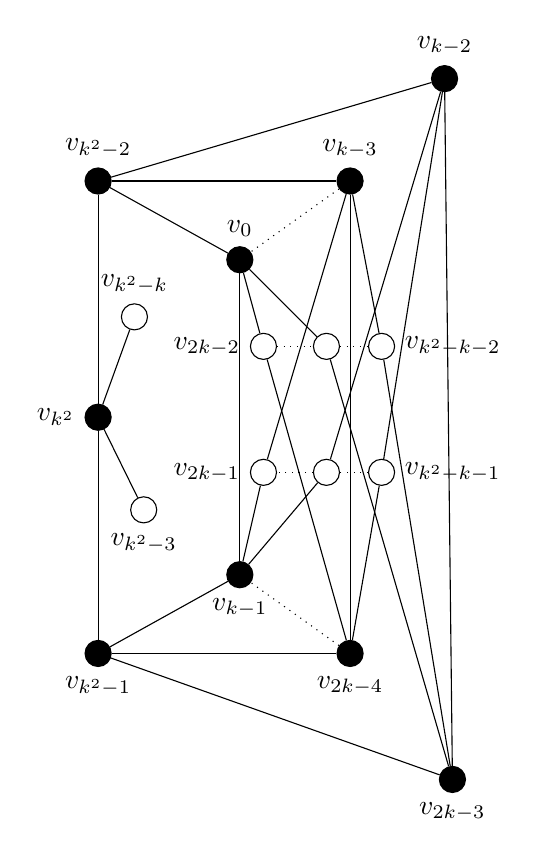
\begin{tikzpicture}
\node[circle,draw,fill,label=$v_{k^2-2}$] (v2) at (-2.5,3) {};
\node[circle,draw,fill,label=$v_{0}$] (v4) at (-0.7,2) {};

\node[circle,draw,fill,label=left:$v_{k^2}$]  (v1) at (-2.5,0) {};
\node[circle,draw,fill,label=below:$v_{k^2-1}$]  (v3) at (-2.5,-3) {};
\node[circle,draw,fill,label=below:$v_{k-1}$] (v7) at (-0.7,-2) {};

\node[circle,draw,fill,label=$v_{k-3}$] (v5) at (0.7,3) {};
\node[circle,draw,fill,label=$v_{k-2}$] (v6) at (1.9,4.3) {};
\node[circle,draw,fill,label=below:$v_{2k-4}$] (v8) at (0.7,-3) {};
\node[circle,draw,fill,label=below:$v_{2k-3}$] (v9) at (2,-4.6) {};

\draw  (v1) edge (v2);
\draw  (v1) edge (v3);
\draw  (v2) edge (v4);
\draw  (v2) edge (v5);
\draw  (v2) edge (v6);
\draw  (v3) edge (v7);
\draw  (v3) edge (v8);
\draw  (v3) edge (v9);
\draw  (v4) edge (v7);
\draw  (v5) edge (v8);
\draw  (v6) edge (v9);

\node[circle,draw,label=$v_{k^2-k}$] (v16) at (-2.0386,1.2748) {};
\node[circle,draw,label=below:$v_{k^2-3}$] (v17) at (-1.921,-1.1761) {};
\draw  (v1) edge (v16);
\draw  (v1) edge (v17);

%\draw[dotted] (v16) edge (v17);
% \draw[dashed] (v4) edge (v8);
% \draw[dashed]  (v5) edge (v7);
% \draw[dashed]  (v6) edge (v7);
% \draw[dashed]  (v4) edge (v9);
% \draw[dashed]  (v5) edge (v9);
% \draw[dashed]  (v6) edge (v8);
% 
\draw[dotted]  (v5) edge (v4);
\draw[dotted]  (v8) edge (v7);

\node[draw,circle,label=left:$v_{2k-2}$] (v10) at (-0.4,0.9) {};
\node[draw,circle,label=left:$v_{2k-1}$] (v11) at (-0.4,-0.7) {};
\node[draw,circle] (v12) at (0.4,0.9) {};
\node[draw,circle] (v13) at (0.4,-0.7) {};
\node[draw,circle,label=right:$v_{k^2-k-1}$] (v15) at (1.1,-0.7) {};
\node[draw,circle,label=right:$v_{k^2-k-2}$] (v14) at (1.1,0.9) {};

\draw  (v4) edge (v10);
\draw  (v10) edge (v8);
\draw  (v7) edge (v11);
\draw  (v11) edge (v5);
\draw  (v4) edge (v12);
\draw  (v9) edge (v12);
\draw  (v7) edge (v13);
\draw  (v13) edge (v6);
\draw  (v5) edge (v14);
\draw  (v14) edge (v9);
\draw  (v8) edge (v15);
\draw  (v15) edge (v6);

\draw[dotted]  (v10) edge (v12);
\draw[dotted]  (v13) edge (v11);
\draw[dotted]  (v12) edge (v14);
\draw[dotted]  (v15) edge (v13);
\end{tikzpicture}
\caption{Fim da etapa-1 de geração do grafo de Moore}
\label{fig-execucao-moore-3}
\end{figure}

Com o esqueleto do grafo gerado na etapa anterior do algoritmo, temos garantidamente um subgrafo do grafo desejado. Partindo desse principio, o Algoritmo \ref{alg-geracao-grafo-moore} é executado, para adicionar arestas aos vértices que ainda não contem $k$ vizinhos, adição das arestas deve ser tal qual a cintura do grafo permaneça 5. Combinações de arestas devem ser testadas a fim de encontrar o grafo respeitando as restrições. Primeiramente os vértices com grau menor que $k$ serão iterados e com uma busca em profundidade, elencando os potenciais vizinhos, 
e a cada iteração um dos vértice de profundidade 4 será escolhido, mantendo a trilha de arestas adicionadas em uma pilha, para uma possível necessidade de se desfazer uma escolha anterior, caso seja identificado que escolha atual resultou em uma combinação inviável ao grafo, e assim poder tentar outras combinações.


\begin{algorithm2e}[h]
\SetAlFnt{\tiny}
\SetAlCapFnt{\small}
\SetAlCapNameFnt{\small}
\SetAlgoLined
\DontPrintSemicolon
\LinesNumbered
\BlankLine
\Entrada{$k$}
\Saida{$G(V_g,E_g)$}
\Inicio{
$V_g \gets \emptyset ;$  $E_g \gets \emptyset$ \\

\ParaCada{$v$ de $0$ até $k^2$}{
  $V_g \gets V_g \cup \{v\} $\\
}

$ k_o \gets k-2 ;$ $ u_v \gets k^2 $\\ %ultimo vertice

\ParaCada{$i$ de $0$ até $k-1$}{
	$E_g \gets E_g \cup \{i,i+k-1\} $\\
}

$ desloc \gets 2 (k - 1) ;$ %desolcamento
$ j_u \gets k(k-1) ;$ %junção
$ ind \gets 0$\\ %indice

\ParaCada{$j$ de $0$ até $k-1$}{
$u \gets j ;$
  $v \gets j + k - 1 ;$  
  $tu \gets u ;$
  $tv \gets v$\\  
  
  \Para{$i$ de $0$ até $k - (2 + j)$}{
    $E_g \gets E_g \cup \{u,desloc\} $\\
    $tv \gets tv + 1$\\
    $E_g \gets E_g \cup \{desloc,tv\} $\\
    $desloc \gets desloc + 1 $\\
    $E_g \gets E_g \cup \{v, desloc\} $\\
    $ind \gets ind + 1 $\\
    $tu \gets tu + 1$\\
    $E_g \gets E_g \cup \{desloc, tu\} $\\
    $desloc \gets desloc + 1 $\\
  }
}
$j_u \gets j_u + k_o $\\
$E_g \gets E_g \cup (j_u, u_v) \cup (u_v, j_u + 1) $\\
\ParaCada{$j$ de $0$ até $k-1$}{
  $u \gets j ;$
  $v \gets j + k - 1 $\\
  $E_g \gets E_g \cup \{j_u, u\} \cup \{j_u +1, v\} $\\
}
$ComplementaArestas(G(V_g,E_g),k)$\\
\Retorna{$G(V_g,E_g)$}
}
\caption{$GeraGrafoMooreD2(k)$}
\label{alg-geracao-grafo-moore}
\end{algorithm2e}

\begin{algorithm2e}[h]
\SetAlFnt{\tiny}
\SetAlCapFnt{\small}
\SetAlCapNameFnt{\small}
\SetAlgoLined
\DontPrintSemicolon
\LinesNumbered
\BlankLine
\Entrada{$G(V_g,E_g),k$}
\Inicio{
 $pilha \gets \emptyset$\\
 $m \gets \frac{(k^2+1)k}{2}$zz
 \Para{$i$ de $0$ até $m$}{
     $lcomb[i] \gets 0$\\
  }
  \Para{$v\in V_g|d(v)<k$}{
    \Enqto{$d(v) < k$}{
       $bfs \gets BFS(G,v)$\\
       $indice \gets |E_g|$\\
       \Se{$d(v) < k$ \textbf{e}  $ \not \exists u\in V_g|bfs(u)=4   $}{
         $retirar(pilha,\{u,w\})$\\
         $E_g \gets E_g \setminus \{u,w\}$\\
          \Para{$i$ de $indice+1$ até $m$}{
     		$lcomb[i] \gets 0$\\
  		  }
         \textbf{continuar enquanto}
       }
       $cont \gets 0$\\
       \Para{$u\in V_g|bfs(u)=4$}{
         \Se{$cont = lcomb[indice]$}{
    	     $E_g \gets E_g \cup \{v,u\} $\\
             $lcomb[indice] \gets lcomb[indice] + 1$\\
             $empurrar(pilha,\{v,u\})$\\
             $\textbf{interromper para}$\\
          }
          $cont \gets cont + 1$\\
       }
     }
  }
}
\caption{$ComplementaArestas(G(V_g,E_g),k)$}%,comb_j)$}
\label{alg-complmenta-arestas}
\end{algorithm2e}

%\section{O Último Grafo de Moore de Diâmetro 2}
A execução do algoritmo com os Parâmetros $k=\{2,3,7\}$ convergiram em poucos segundos para os respectivos grafos $C_5$, Petersen e Hoffman-Singleton. O resultado da execução pode ser conferido na Tabela~\ref{tabela-implementacao-moore}. E uma versão do algoritmo implementada em \textit{Java} está disponível juntamente com todos os códigos deste trabalho, conforme será descrito no próximo capítulo. 

Na execução do algoritmo anterior com o parâmetro $k=57$, a execução otimizada do mesmo não convergiu a tempo da finalização deste trabalho, ainda permanecendo em aberto a sua existência. Porém conseguimos obter o esqueleto de seu subgrafo, que dado o tamanho optamos por não disponibilizar neste texto, o mesmo pode ser encontrado junto aos códigos disponibilizados, como \textit{esqueleto-ultimo-grafo-moore.es} e a situação atual do processamento do grafo no fechamento deste trabalho como \textit{maior-complemento-ultimo-grafo-moore.es}. Que até o fechamento deste constavam menos da metade das arestas restantes, podendo ser utilizado em futuros trabalhos, pra quem busca encontrá-lo seguindo o mesmo caminho.

No próximo capítulo iremos abordar as implementações realizadas neste trabalho.


\begin{table}[h]
\caption{Lista de arestas resultante do Algoritmo~\ref{alg-geracao-grafo-moore} para $k=\{2,3,7\}$}
\label{tabela-implementacao-moore}
\centering
\begin{tabular}{|r|p{1cm}|p{2cm}|p{8cm}|}
\hline
\textbf{K}  & \textbf{2} & \textbf{3} & \textbf{7} \\ \hline
 \rotatebox[origin=c]{90}{\textbf{Esqueleto }}   & 2-4, 4-3, 2-0, 3-1, 0-1 & 7-9, 9-8, 7-0, 8-2, 7-1, 8-3, 0-2, 1-3, 0-4, 4-3, 2-5, 5-1, 9-6 & 47-49, 49-48, 47-0, 48-6, 47-1, 48-7, 47-2, 48-8, 47-3, 48-9, 47-4, 48-10, 47-5, 48-11, 0-6, 1-7, 2-8, 3-9, 4-10, 5-11, 0-12, 12-7, 6-13, 13-1, 0-14, 14-8, 6-15, 15-2, 0-16, 16-9, 6-17, 17-3, 0-18, 18-10, 6-19, 19-4, 0-20, 20-11, 6-21, 21-5,  1-22, 22-8, 7-23, 23-2, 1-24, 24-9, 7-25, 25-3, 1-26, 26-10, 7-27, 27-4, 1-28, 28-11, 7-29, 29-5,  2-30, 30-9, 8-31, 31-3, 2-32, 32-10, 8-33, 33-4, 2-34, 34-11, 8-35, 35-5, 3-36, 36-10, 9-37, 37-4, 3-38, 38-11, 9-39, 39-5, 4-40, 40-11, 10-41, 41-5, 49-42, 49-43, 49-44, 49-45, 49-46 \\ \hline
\rotatebox[origin=c]{90}{\textbf{Complemento }} &                         & 4-6,5-6                                                         & 12-30, 12-35, 12-36, 12-40, 12-42, 13-31, 13-34, 13-37, 13-41, 13-42, 14-24, 14-27, 14-38, 14-41, 14-43, 15-25, 15-26, 15-39, 15-40, 15-43, 16-26, 16-29, 16-33, 16-34, 16-44, 17-27, 17-28, 17-32, 17-35, 17-44, 18-23, 18-28, 18-31, 18-39, 18-45, 19-22, 19-29, 19-30, 19-38, 19-45, 20-22, 20-25, 20-32, 20-37,  20-46, 21-23, 21-24, 21-33, 21-36, 21-46, 22-36, 22-39, 22-44, 23-37, 23-38, 23-44, 24-32, 24-40, 24-45, 25-33, 25-41, 25-45, 26-35, 26-38, 26-46, 27-34, 27-39, 27-46, 28-30, 28-33, 28-43, 29-31, 29-32, 29-43, 30-41, 30-46, 31-40, 31-46,  32-42, 33-42, 34-45, 34-36, 35-37, 35-45, 36-43, 37-43, 38-42, 39-42, 40-44, 41-44   \\ \hline
\end{tabular}
\end{table}


